\chapter{Five Beginner Entrepreneurial Moves}

This chapter follows a School of Hard Knocks entrepreneurship lesson curated by LazyingArt LLC through Video2Book. The source is a trail-walk talk rather than a board lecture, so the mathematics here is deliberately modest: not invented blackboard work, but compact notation for the business mechanisms the speaker actually describes. We keep the lecture's order. First comes the founder's reason for continuing, then the cash needed to survive, and only then the five operating moves: sales, accounting, onboarding, content, and networking.

\section{A Trail Walk Instead of a Boardroom}

The speaker begins by changing the setting. He says this will be a walk rather than the usual serious business or finance video. That is not a throwaway detail. It tells us how to read the whole lecture. The advice is not presented as abstract doctrine; it is practical hindsight, the sort of direct counsel a person might give to a younger version of himself.

So we should not flatten the lesson into a generic list. Its order matters. The speaker first asks what keeps a founder going, then what keeps the founder funded, and only after that does he enter the numbered tips. In compressed form, the lecture moves like this:
\[
\begin{aligned}
\text{reason to continue}
&\longrightarrow \text{cash runway} \\
&\longrightarrow \text{sales} \\
&\longrightarrow \text{financial visibility} \\
&\longrightarrow \text{customer stability} \\
&\longrightarrow \text{relationship leverage}.
\end{aligned}
\]
This is a reconstruction of the spoken sequence, not a formula from a board. Its purpose is to keep the chapter faithful to the lecture's rhythm: survival before scale, then operating discipline.

\section{Before the Tips: Why and Cash Runway}

Before the numbered list begins, the speaker pauses on what he calls more important than the tips themselves: figuring out one's ``why.'' The point is not motivational decoration. It is a claim about persistence under noisy feedback. Some days the business feels easy. Other days nothing seems to work, and negative self-talk asks why the founder is working so hard without seeing results.

A cautious way to write the mechanism is
\[
M_{t+1} \approx M_t + Y_t - D_t,
\]
where \(M_t\) is the founder's commitment at time \(t\), \(Y_t\) is the reinforcing effect of the founder's reason for continuing, and \(D_t\) is discouragement from bad days, stalled progress, or self-doubt. The speaker does not give this model explicitly. It is a compact way of saying what his narration says in plain language: if discouragement is real, the founder needs a durable reason that can absorb it.

\subsection{Question \& Answer}

\paragraph{Question.}
If the business is not yet producing visible results, why keep working so hard?

\paragraph{Answer.}
The speaker's answer is that the founder's ``why'' carries part of the load before the market gives clean evidence. This does not mean motivation replaces customers, revenue, or financial discipline. It means early entrepreneurship contains intervals where feedback is delayed or discouraging, and a founder needs a reason strong enough to continue through those intervals.

He then makes the second pre-tip point: it is perfectly acceptable to work a job while starting a business. Rent, food, and ordinary living costs do not disappear because a person has begun a company. In notation, the beginner's survival constraint is
\[
W_t + B_t \geq R_t + F_t + P_t,
\]
where \(W_t\) is wage or job income, \(B_t\) is available business or startup cash, \(R_t\) is rent, \(F_t\) is food, and \(P_t\) represents other personal living costs. If the left side is too small, the founder does not have enough runway.

\subsection{Question \& Answer}

\paragraph{Question.}
Is working a job a contradiction of entrepreneurship?

\paragraph{Answer.}
No. In the speaker's framing, a job can be the funding mechanism that keeps the founder alive and, where possible, lets money be injected into the business. The job is not romantic, but it can be structurally useful:
\[
W_t
=
\text{living support}
+
\text{possible business injection}.
\]
The practical point is sober: a young business may not yet be profitable enough to support its owner. Working while building can be a constraint solution, not a failure of ambition.

\section{Tip One: Sales as the Golden Rule}

Only the first tip is given priority. The remaining tips are in no particular order, but this one is called a golden rule: know sales. The speaker states the commercial condition directly. If the founder cannot sell people into buying the product or service, then there is no business.

We can write the implication as
\[
\text{no ability to sell}
\;\Longrightarrow\;
\text{no functioning business}.
\]
This is not a theory about personality. It is a theory about exchange. A business needs customers who actually buy.

The speaker then adds the pressure of churn. Customers leave. Customer turnover is real. Therefore, selling is not a one-time launch event; it is a continuing requirement. Let
\[
\begin{aligned}
C_t &= \text{customers at time } t, \\
N_t &= \text{new customers acquired during period } t, \\
L_t &= \text{customers lost during period } t.
\end{aligned}
\]
A minimal customer-base update is
\[
C_{t+1}\approx C_t+N_t-L_t.
\]
The condition for growth is then
\[
C_{t+1}>C_t
\quad\Longleftrightarrow\quad
N_t>L_t.
\]
That is the mathematical skeleton of the speaker's warning that if the business is not growing, it is dying. Churn is a subtraction term, so marketing and sales have to keep adding.

\subsection{A Worked Customer Example}

Suppose a small service business begins the month with \(C_t=40\) active customers. It gains \(N_t=8\) new customers and loses \(L_t=5\) customers. Then
\[
C_{t+1}\approx 40+8-5=43.
\]
The business grew by three customers.

If the same business gains only \(N_t=3\) customers while losing \(L_t=5\), then
\[
C_{t+1}\approx 40+3-5=38.
\]
The business may still feel busy, but the base is shrinking. That is why the speaker treats sales as maintenance as well as growth.

\section{Training Sales Like an Athlete}

The sales section then turns into a mentor story. The speaker recalls Joe Soto telling him to stop ``playing with my food.'' In context, the phrase means he was walking into sales presentations and demos without practicing his pitch.

The analogy is a professional athlete. An athlete practices, watches film, and corrects performance. The speaker says a salesperson should do the same: role play, practice the pitch, watch or rewatch meetings, listen to the way the conversation sounds, and improve how difficult scenarios are handled.

\[
\begin{aligned}
\text{attempt}
&\longrightarrow \text{review} \\
&\longrightarrow \text{practice} \\
&\longrightarrow \text{corrected attempt}.
\end{aligned}
\]

\begin{figure}
\centering
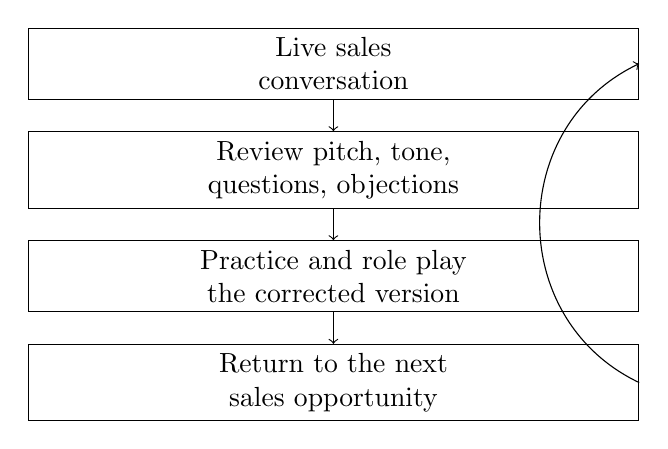
\begin{tikzpicture}
\node[draw, align=center, text width=0.62\linewidth] (a) at (0,0) {Live sales\\conversation};
\node[draw, align=center, text width=0.62\linewidth] (b) at (0,-1.35) {Review pitch, tone,\\questions, objections};
\node[draw, align=center, text width=0.62\linewidth] (c) at (0,-2.70) {Practice and role play\\the corrected version};
\node[draw, align=center, text width=0.62\linewidth] (d) at (0,-4.05) {Return to the next\\sales opportunity};
\draw[->] (a) -- (b);
\draw[->] (b) -- (c);
\draw[->] (c) -- (d);
\draw[->] (d.east) .. controls (2.2,-3.25) and (2.2,-0.80) .. (a.east);
\end{tikzpicture}
\caption{A transcript-derived sales practice loop. The point is that sales improves through feedback, not merely through exposure.}
\end{figure}

The important distinction is between doing more calls and training from the calls. Exposure gives repetitions. Training adds review, correction, and deliberate return.

\section{Tip Two and Tip Three: Accounting, Then Onboarding}

Tip two is accounting. The speaker presents it as advice to his younger self, because he says he made poor financial decisions when he did not understand accounting or how the numbers worked in business. The chapter should keep this simple. The claim is not that a beginner must become a professional accountant. The claim is that basic accounting narrows the gap between impression and reality:
\[
\begin{aligned}
\text{felt condition of the business}
&\neq \\
&\text{measured condition of the business}.
\end{aligned}
\]
Accounting is the discipline that tells the founder where the business actually is, rather than where the founder hopes it is.

The lecture then shifts, with the hiking aside left intact in spirit, to tip three: customer onboarding. The question is what happens after someone purchases from the business. That is a precise operational pivot. Sales gets the customer in the door; onboarding determines whether the customer feels confident after entering.

\subsection{Question \& Answer}

\paragraph{Question.}
Is the sale the end of the customer problem?

\paragraph{Answer.}
No. The sale begins a new interval of risk. The customer can experience buyer's remorse, misunderstand the service relationship, or become unhappy with unclear communication. The speaker focuses on two concrete dangers: a chargeback soon after purchase and future problems caused by poorly set expectations.

A useful onboarding system therefore makes the next state explicit:
\[
\begin{aligned}
\text{purchase}
&\longrightarrow \text{reassurance} \\
&\longrightarrow \text{expectations} \\
&\longrightarrow \text{next steps}.
\end{aligned}
\]
The operational effect is
\[
\begin{aligned}
\text{clear onboarding}
&\longrightarrow \text{less remorse} \\
&\quad + \text{clearer expectations} \\
&\quad + \text{fewer avoidable conflicts}.
\end{aligned}
\]
Again, this is a mechanism rather than a guarantee. It says where the work of retention begins.

\begin{figure}
\centering
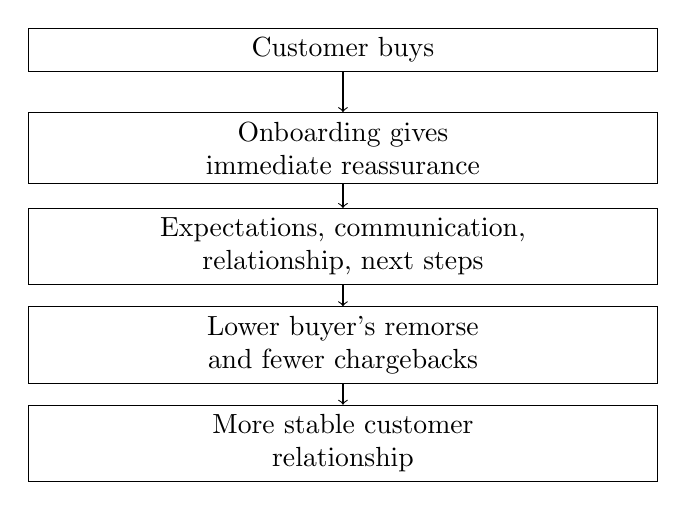
\begin{tikzpicture}
\node[draw, align=center, text width=0.64\linewidth] (a) at (0,0) {Customer buys};
\node[draw, align=center, text width=0.64\linewidth] (b) at (0,-1.25) {Onboarding gives\\immediate reassurance};
\node[draw, align=center, text width=0.64\linewidth] (c) at (0,-2.50) {Expectations, communication,\\relationship, next steps};
\node[draw, align=center, text width=0.64\linewidth] (d) at (0,-3.75) {Lower buyer's remorse\\and fewer chargebacks};
\node[draw, align=center, text width=0.64\linewidth] (e) at (0,-5.00) {More stable customer\\relationship};
\draw[->] (a) -- (b);
\draw[->] (b) -- (c);
\draw[->] (c) -- (d);
\draw[->] (d) -- (e);
\end{tikzpicture}
\caption{A transcript-derived onboarding chain. After the purchase, the business has to stabilize the customer's decision.}
\end{figure}

\section{Tip Four: Content, Social Media, and Referral Leverage}

Tip four is investing in content and social media. The speaker's reasoning begins with attention: people spend time on social media, especially at home and on their phones. A beginner business can use that attention by sharing useful content, meaningful updates, and evidence of progress.

He especially emphasizes the people already close to the founder: friends, family, and people the founder knows. The transcript phrase is not perfectly clean, but the mechanism is clear enough. A beginner does not need a national audience before social media matters. The first useful audience may be the immediate network.

Then the lecture gives a concrete anecdote. The speaker describes Austin Smith, a digital marketing owner, holding up a stack of cash and offering payment for referrals to business owners who could benefit from his services. According to the speaker, Austin gave away \(\$10{,}000\), and the video helped him close probably close to \(\$100{,}000\) worth of business after going viral locally.

The numbers should be preserved with the speaker's uncertainty:
\[
\begin{aligned}
\text{claimed giveaway} &= \$10{,}000, \\
\text{claimed closed business} &\approx \$100{,}000.
\end{aligned}
\]
The rough gross comparison is
\[
\frac{\$100{,}000}{\$10{,}000}\approx 10.
\]
This is not net profit, audited return, or a promise that any referral offer produces the same result. It is an anecdotal gross multiple. The mechanism is the important part:
\[
\begin{aligned}
\text{clear referral offer}
&+ \text{local attention} \\
&+ \text{credible incentive} \\
&\longrightarrow \text{introductions} \\
&\longrightarrow \text{closed business}.
\end{aligned}
\]

\section{Tip Five: Networking by Investing in Other People}

The fifth tip is networking, but the speaker immediately separates useful networking from shallow networking. The shallow version is to hand out business cards and try to sell one's own products and services. The recommended version is to invest in other people's stories.

That means asking about their products, services, and reasons for doing what they do. It also means giving free advice or free value when possible. The payoff may not be immediate. The speaker describes a delayed effect: someone may remember the interaction two months later and make an introduction.

A compact relationship model is
\[
\begin{aligned}
\text{attention to another person}
&+ \text{useful free value} \\
&\longrightarrow \text{memory and trust} \\
&\longrightarrow \text{future referral}.
\end{aligned}
\]
This is why the speaker calls networking a matter of planting seeds. The commercial effect is delayed, but the relationship path has been opened.

The book recommendations at the end of the section fit this same logic. \emph{How to Win Friends and Influence People} and \emph{Giftology} are named as resources for building a better network. In the structure of the lecture, they point back to the same mechanism: relationships are not side chatter around the business; they are part of how opportunity travels.

\section{Summary}

The talk is informal in setting, but disciplined in sequence. First we need a reason to continue and enough cash runway to keep the founder alive. Then we need sales, because without buyers there is no business. Sales must be trained through review and correction. Accounting gives the founder a measured view of the business. Onboarding protects the relationship after purchase. Content uses attention as leverage. Networking uses generosity, memory, and trust as relationship leverage.

The working equations are reconstructions of the business logic, not visible board mathematics:
\[
W_t+B_t\geq R_t+F_t+P_t,
\]
\[
C_{t+1}\approx C_t+N_t-L_t,
\]
and
\[
N_t>L_t.
\]
Together they express the lecture's practical spine: fund the founder, keep new customers arriving faster than old customers leave, and build systems that let effort become repeatable business.
